\documentclass{llncs}

\usepackage{graphicx}
\usepackage[english]{babel}
\usepackage{float}
\usepackage[unicode=true,bookmarks=true,bookmarksnumbered=false,bookmarksopen=false,breaklinks=false,pdfborder={0 0 0},backref=false,colorlinks=false]{hyperref}
\hypersetup{pdftitle={Park Assistant}, pdfauthor={Matteo Ragni -
161822},pdfsubject={Homework 02}}

\usepackage{amsmath}

\usepackage{listings}
\usepackage{color}

\definecolor{dkgreen}{rgb}{0,0.6,0}
\definecolor{gray}{rgb}{0.5,0.5,0.5}
\definecolor{mauve}{rgb}{0.58,0,0.82}

\lstset{frame=tb,
  language=C++,
  aboveskip=3mm,
  belowskip=3mm,
  showstringspaces=false,
  columns=flexible,
  basicstyle={\small\ttfamily},
  numbers=none,
  numberstyle=\tiny\color{gray},
  keywordstyle=\color{blue},
  commentstyle=\color{dkgreen},
  stringstyle=\color{mauve},
  breaklines=true,
  breakatwhitespace=true
  tabsize=3
}

% Definitions of newcommand

% Insert a new figure in the document, inside a float.
\newcommand{\fig}[4]{
	% /fig{image file}{caption}{scaling factor}{label name} 
	% 1 - FILE IMAGE										
	% 2 - CAPTION OF THE IMAGE								
	% 3 - SCALING FACTOR									
	% 4 - LABEL NAME										
	\begin{figure}[H] \label{#4}
		\centering
		\includegraphics[keepaspectratio, scale=#3]{#1}
		\caption{#2}
	\end{figure}
}






\begin{document}


\title{Park Assistant}

\author{Matteo Ragni, [161822]}

\institute{Computer Vision, University of Trento}
\maketitle

% Abstract
\begin{abstract}
In this work will be presented some alghoritms that identify free spots in parking lot. 
The alghoritms are parametric, do not need an image af the complete parking lot free, 
and some insight to improve them are presented in the different chapter. In the first 
part we will get some insight of the system that divide the single parking spot from 
the whole image, and than we will analize the two different alghoritms used to
get the \emph{status} of a spot.

Must be taken into account the didactical natur of this project. Optimization is
put aside, while the largest different solutions are used to obtain the final
result. This is one of the main reason that brought us to write a code that uses
two different solutions for initialization and for real time processing.

\end{abstract}

% Chapter 1: General situation analisys
%  - Analysis of the images and problems to face
%  - Subdivision of the parking spot and warping
%% CHAPTER 1

\section{General Situation Analysis}

	\subsection{Analysis of the Problem}
	
		The images are taken from a fixed camera. Making the difference between two
		frames is evident that camera has some little oscillations, but in general we
		could state a formal hypothesis of fixed camera, on which we will base all the
		analysis.
		
		There are some little problem that should be taken into account:
		\begin{itemize}
		  \item illumination may change during daytime, so the algorithm should be
		  robust against some of the derived problems, like shadows and reflections;
		  \item parallax is another problem with some relevance; over a certain angle
		  between camera axis and park spot, even the more robust algorithm will fail
		  because of the occlusions of the other parked cars.
		  \item there are some conclusions to derive for a bad parked car; if the car
		  occupy two parking spot, the algorithm must consider both spot busy, while if
		  one of the two park spot could be considered free, and another car may park,
		  the algorithm should report it as free;
		  \item occlusions: we have already touched this point, but some object may
		  occlude some parking spot, i.e. a street lamp between the camera and the
		  observed park spot.
		\end{itemize}
		
		For this problem we could derive some simple answer that generally speaking
		should be implemented:
		\begin{itemize}
		  \item The illumination problem could be bypassed using some different color
		  space, like the HSV and transforming the image in gray-scale.
		  \item The problem of the parallax make the use of rectangles to select a
		  park spot not a robust solution. When the parallax is to high, the only
		  feasible solution is to make use of another camera, because the problem will fall in a
		  problem of occlusion. If the parallax is not too high, the right answer is to
		  make use of a warping transformation, related to the four corner of the
		  single parking spot. This make the algorithm more robust also to the bad
		  parked car (see \ref{sub:warping}).
		  \item For small occlusions the only feasible solution is to create
		  different parameter for each park spot, that should be calibrated with
		  respect to its characteristics (occlusion as a characteristic). For very big
		  occlusions there is only one solution: change the camera's point of view.
		\end{itemize}
	
	\subsection{The Parking Spot}
	
		\subsubsection{The Parking Spot Object}
		
			The single parking spot object is initialized with a configuration file. The
			initialization follow this syntax:
			\begin{verbatim}
	%YAML:1.0
	parking_spot: 22
	spots: 
	[...]
	 - { nspot:2,  rect:[80,  427, 35, 37], 
	     polyx:[70,  118, 135,  93], 
	     polyy:[466, 465, 427, 424], 
	     param:[20000,30000,4,13,1] }
	[...]		
			\end{verbatim}
			where \verb+parking_spot+ is a global variable that will give the total number
			of parking spot that should be tracked, and \verb+spots+ is a list of
			associative arrays. In each associative array there are some variables that
			will be used in the code. The variable \verb+nspot+ is an id for the parking
			spot, \verb+rect+ is an array that represent a rectangle ($x$ top left
			position, $y$ top left position, width and height - this variable is
			currently unused). The variables \verb+ployx+ and \verb+polyy+ are two arrays
			that represent the four corner of a single parking spot. This point should be
			ordered, to create polylines. \verb+param+ is an ordered array of parameter
			used in different algorithms. 
			
			The \verb+ParkSpotObj+ is the class that represent a single parking spot,
			while the collection of the whole parking is a vector of object of that class.
			In the class, variables and methods are implemented to make the single park
			spot self-contained. Some algorithms implemented inside the object are:
			\begin{itemize}
			  \item initialization;
			  \item warping functions (see \ref{sub:warping});
			  \item some histograms operations, using the class \verb+Histogram+ that
			  implement some useful implementations to evaluate histograms component of
			  an image;
			  \item edge detection methods;
			  \item plotting and printing information on current frame or on
			  \verb+stdout+.
			\end{itemize}
		
		\subsubsection{The warping algorithm \label{sub:warping}}
		
		As we said before, to get as much information as possible we have to transform
		the quadrilateral parking spot (as perceived by the camera) in a rectangular
		image on which we could make some calculations.
		
		Given the four source corner $\mathbf{s_i}$ and the four destination corner
		$\mathbf{d_i}$, the transformation matrix is given by the solution of the
		equations:
		
		\begin{equation}
			\mathbf{d_i} - \mathbf{T}\times\mathbf{s_i} = 0 \qquad
			\mathrm{for}\,i=1,\ldots,4
		\end{equation}
		
		In particular, the code chose automatically the destination points on the
		basis of the bigger rectangle that contains the initial quadrilateral park
		spot. Once resolved $\mathbf{T}$, the transformation to extract the single,
		given a source matrix $\mathbf{S}$ and a destination matrix $\mathbf{D}$ is:
		
		\begin{equation}
			\mathbf{D}(x,y) = \mathbf{S}\left(
			\dfrac{T_{1,1}x+T_{1,2}y+T_{1,3}}{T_{3,1}x+T_{3,2}y+T_{3,3}},
			\dfrac{T_{2,1}x+T_{2,2}y+T_{2,3}}{T_{3,1}x+T_{3,2}y+T_{3,3}} \right)
		\end{equation}
		
		The optimization of this part of good is quite good. The transformation matrix
		is generated once, by the object constructor, while the transformation is
		called each frame by the \verb+ParkSpotObj::refreshImage()+ method (and
		similar).
		
		\begin{figure}[H] \label{fig:warping}
			\centering
				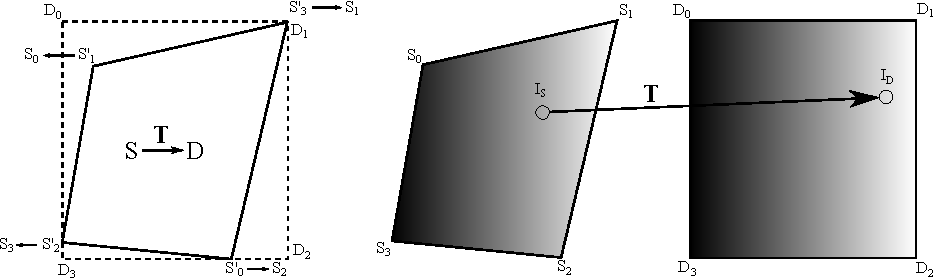
\includegraphics[keepaspectratio, scale=0.6]{img/warping.pdf}
			\caption{Representation of the warping algorithm}
		\end{figure}

% Chapter 2: Initialization of the system
%  - Analysis of the image in the HSV space
%  - Writing down the classifier. Implementing it in class ParkSpot
%% CHAPTER 2
% Initialization of the system
%  - Analysis of the image in the HSV space
%  - Writing down the classifier. Implementing it in class ParkSpot

\section{Initialization of the System}

	\subsection{Classification with Histograms}
	
	Here is presented the algorithm used to initialize the system. The algorithm is
	a classifier developed upon the classification of two main parameters that
	tends to separate busy parking spot, from free ones. 
	
	Taken an image converted in HSV color space, we could extract the mean and the
	standard deviation for each component. The plot of the standard
	deviation of the Saturation components against the mean of Value component, for
	a single frame, will give us this single situation. Parking spot status is
	known, and we can see a strong separation (see figure \ref{fig:separate}, on
	the left).
	
	The two different status could be separated with two degrees of freedom of a
	line. The inclination and offset of the line could be used to derive
	rotation plus translation equation that will help us to discriminate between
	the busy and the free parking spot. Given a point ${\sigma_{2},\mu_{3}}^{T}$, and a
	separation line in the form $\mu_{3} = \alpha \sigma_{2}+\eta$, we could derive
	this transformation:
	\begin{equation}
		\left\{ \begin{array}{c}
\xi_{1}\\
\xi_{2}
\end{array}\right\} =\left[\begin{array}{cc}
\cos(\alpha) & \sin(\alpha)\\
-\sin(\alpha) & \cos(\alpha)
\end{array}\right]\left\{ \begin{array}{c}
\sigma_{2}\\
\mu_{3}
\end{array}\right\} -\left\{ \begin{array}{c}
1\\
1
\end{array}\right\} \eta
	\end{equation}
	the algorithm has only to check:
	\begin{equation}
		\xi_{2} \geq 0
	\end{equation}
	if this condition is true, than the park spot is busy, else the parking spot is
	free.
	% TODO Figura separazione singola e rispetto al tempo label: fig:separate
	\begin{figure}[H] \label{fig:separate}
		\centering
			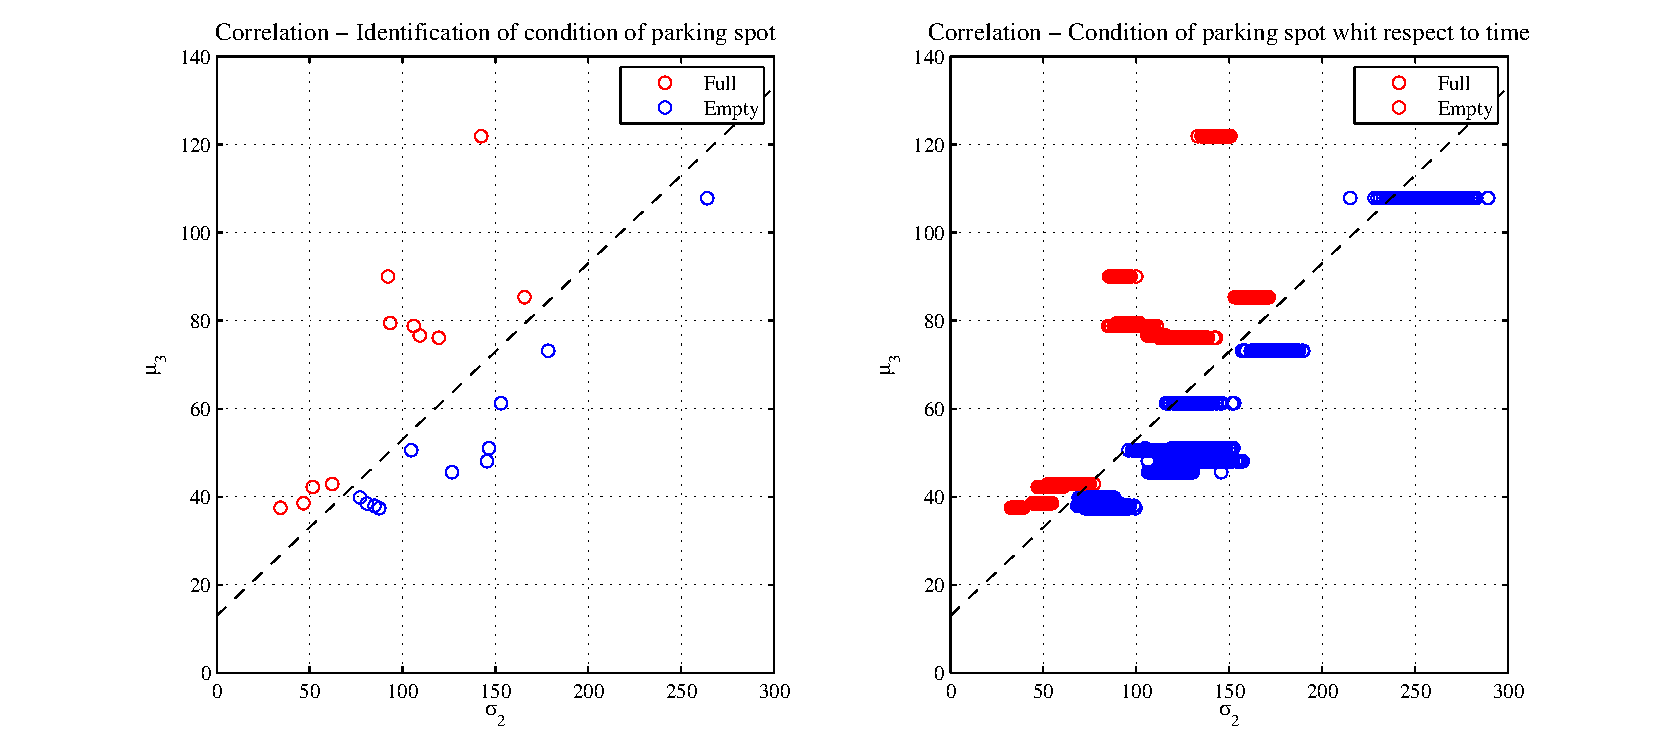
\includegraphics[keepaspectratio, scale=0.4]{img/img1.pdf}
		\caption{Classifier data in 2D representation}
	\end{figure}
	
	Referring to the image on the right, in figure \ref{fig:separate}, it is easy
	to understand that this classification is not robust in time, if not
	expanded with tuning of the parameters each frame (learning
	algorithm). Means tend to remain almost equal, but standard deviations tend to
	change in time. The learning method should change the angle of the separation
	line (and also the discrimination algorithm) to get a good classification. We
	have decided to leave this method, for something that is little more 
	sophisticated, and to discover more about the \verb+openCV+ libraries.
	
	As a drawback, we can also consider the fact that there will be no control on
	the evolution of the classifier discrimination parameters.
	
	\subsection{Diving in the Code}
	In the code, this initialization script is called when a new object
	\verb+ParkSpotObj+ is created, as \verb+int ParkSpotObj::initialStatus()+
	method. The projection of the two characteristics is made by the single object,
	to follow the self-containment philosophy. The parameters that drive the
	algorithm are the number 3 and 4 in the \verb+param+ element of the
	configuration script.
	
	The code is almost at a good level of optimization, because the number of bins
	extracted for the histograms are 32, and the area on which is evaluated the
	status is relatively small.


% Chapter 3: The real time alghoritm
%  - The edge detector as identifier
%  - The MOG as movement detector: a switch for the identifier
%% Chapter 3: The real time alghoritm
%  - The edge detector as identifier
%  - The MOG as movement detector: a switch for the identifier

\section{Real Time Application}

	\subsection{Edge and MOG: the Rude Approach}
	
	The real time application follow a different approach, that has some advantages
	and some drawbacks. Two algorithms runs in parallel, to understand the status
	of the parking. The first algorithm, that is a mixture of gaussians, is used to
	identify a movement on the single parking spot. When a movement is detected, it
	enables the execution of the second algorithm, that is a Canny edge detector.
	The result of the edge detector (gray-scale image, due to linear perspective
	transformation) is summed up on the area of the single park spot, and if it
	reach a certain threshold (in configuration file the first element of
	\verb+param+).
	
	While there is movement on a parking spot, the system set its state to
	\emph{wait}, to make the user understand that it cannot derive conclusions on
	its state.
	
	The MOG system is calibrated with a really low learning rate ($\alpha = 0.1$)
	and for each pixel 3 gaussians model are generated. The Canny edge detection
	has an high threshold, and uses a Sobel kernel of dimension $3\times3$.
	
	The threshold value was derived analyzing a set of collected data, over time.
	The separation is almost obvious.
	
	% TODO inserire figura che spiega come funziona algoritmo a sinistra e a destra
	% la calibrazione dell'algoritmo (devo scaricare il file!)
	\begin{figure}[H] \label{fig:mog}
		\centering
			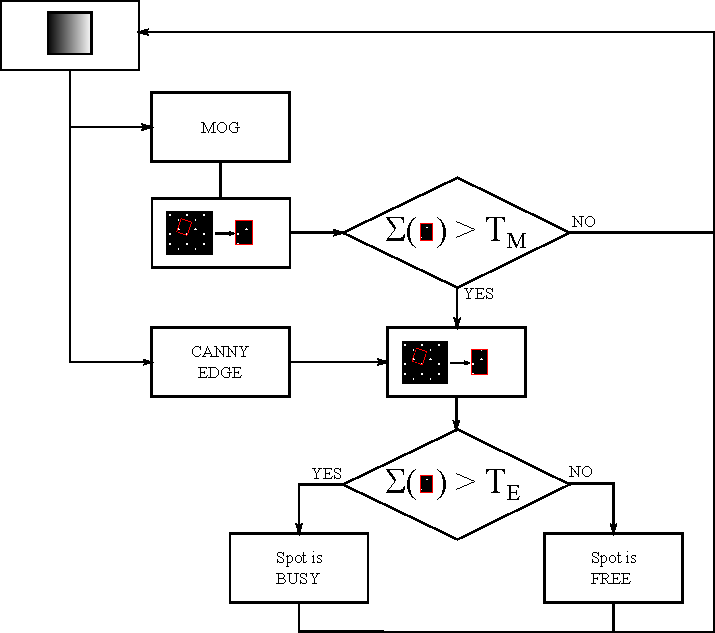
\includegraphics[keepaspectratio, scale=0.55]{img/mogandedge.pdf}
			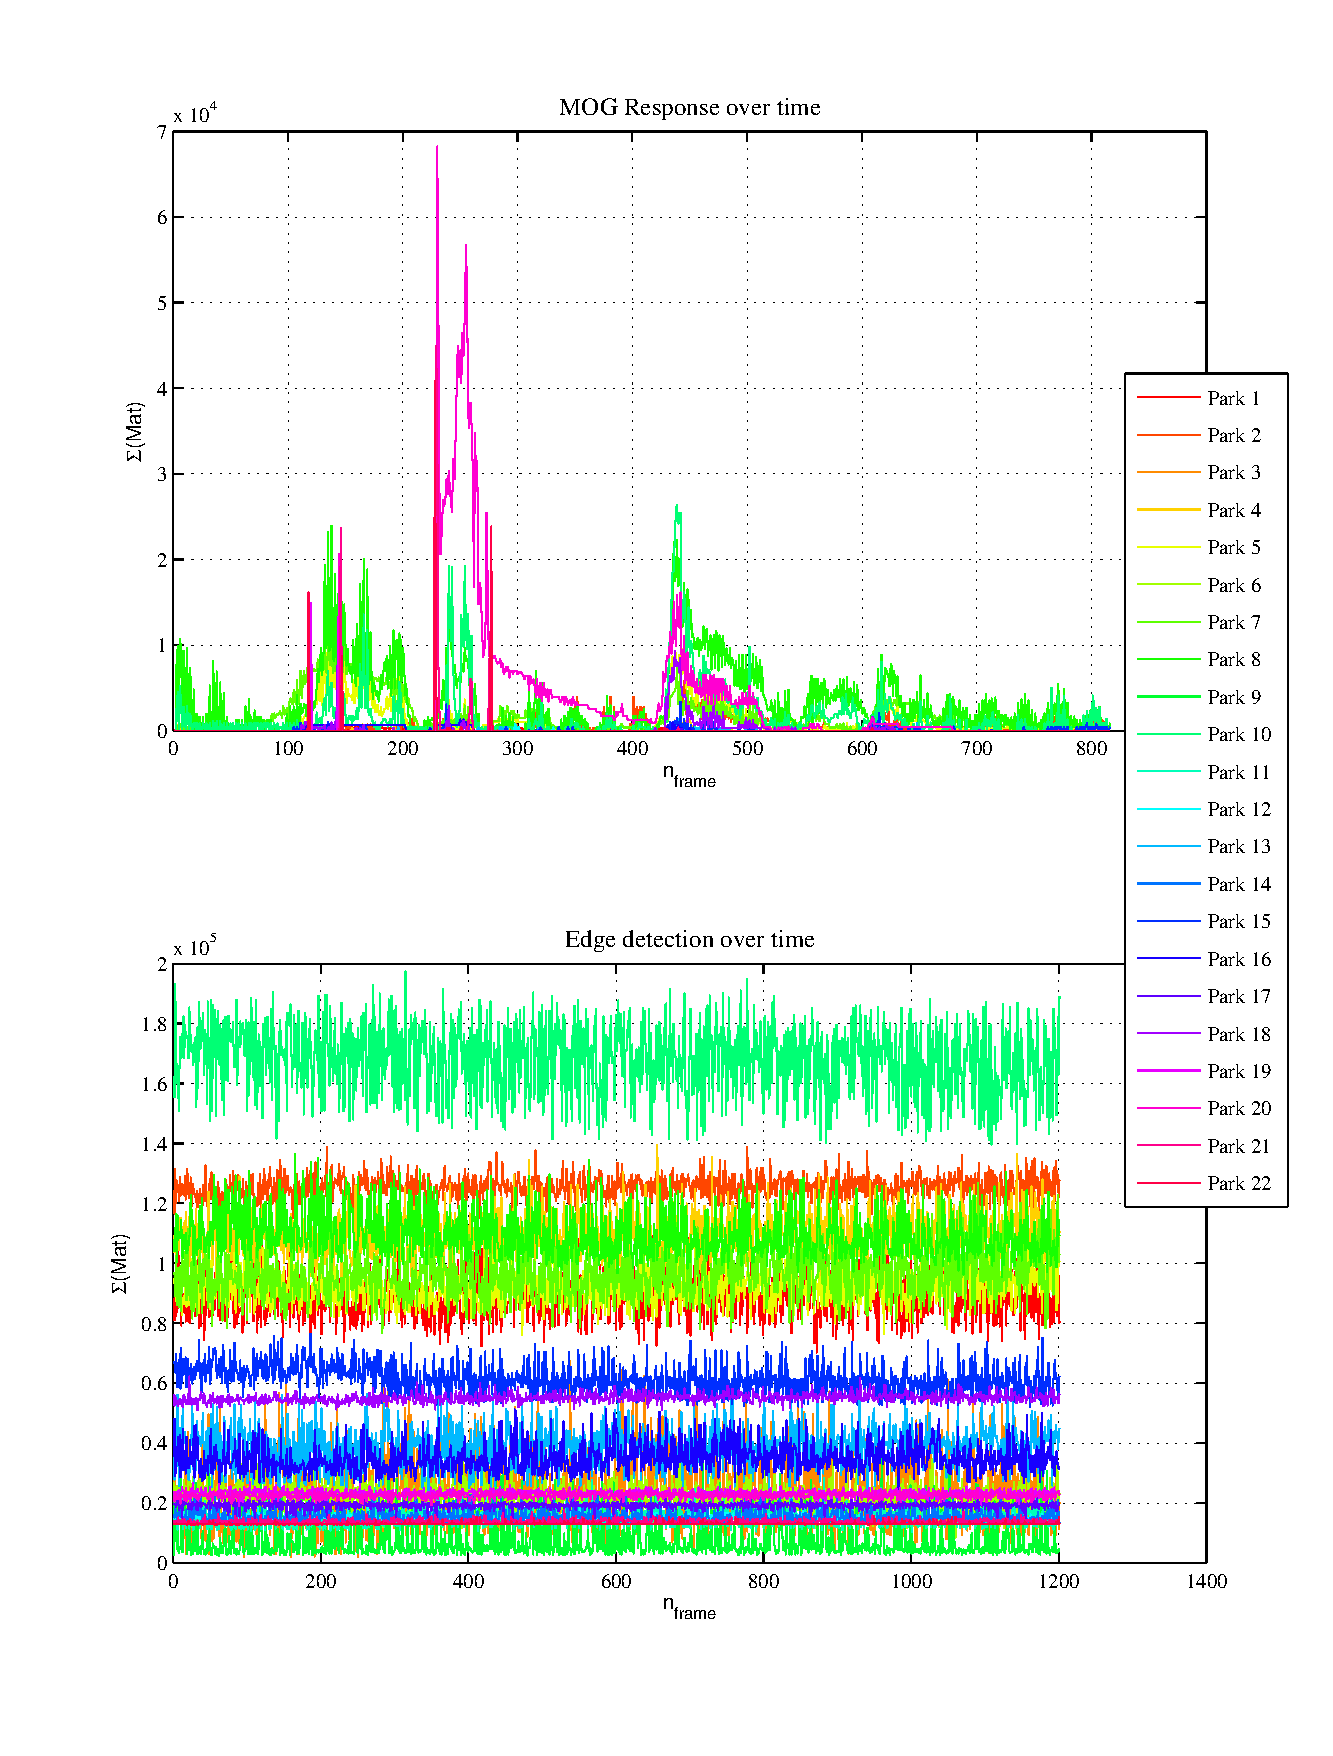
\includegraphics[keepaspectratio, scale=0.2]{img/img2.pdf}
		\caption{The combination of MOG and Canny Edge algorithms}
	\end{figure}
	
	\subsection{Drawbacks}

	This implementation seems to work quite well, but for sure it is not an optimal
	solution. For each frame, a mixture of gaussians and a Canny algorithm, that
	have both an high computational load, run on the whole set of pixels. So we can
	count:
	\begin{itemize}
	  \item extremely high computational load.
	  \item this system is not robust against illumination: sometimes the shadows
	  could bring to a formation of fake edges that could be bring the system to
	  interpret the parking spot as busy. The good point 
	\end{itemize}
	
\section{Conclusions}

	There are a lot of improvements that could be added to make this code better,
	but the first should be the optimization of the code. There are several point
	that need to be revised:
	\begin{itemize}
	  \item On each frame, for each pixel, both edge detection and MOG runs on the
	  whole image area. The code needs to be modified for an extraction
	  and execution of the algorithm on the littler area. This means add a support
	  for relative coordinates.
	  \item Elimination of unused variables. Some of the code was written for
	  support standard \verb+Rect+ instead of a polygonal area. Those part should
	  be removed from the code to make it lighter.
	  \item Add a stronger use of pointer for \verb+Mat+ in functions. Actually a
	  lot of functions receives as variables the whole \verb+Mat+ instead of a more
	  lighter pointer.
	\end{itemize}
	From the algorithmic point of view, the two methods must be joined to work
	together: the edge detection, launched by the MOG movement detector, should
	have more than one threshold, one higher that represents the highest
	probability that the place is busy, one lower that represents the lowest
	probability that the place has a car parked in. While the edge get a result in
	between this two thresholds, the histograms classifier will be invoked to make
	a last classification. In this way we exploit the illumination weaknesses of
	the edge detector and the training weakness of the classifier.
	
	\begin{figure}[H] \label{fig:final}
	\centering
		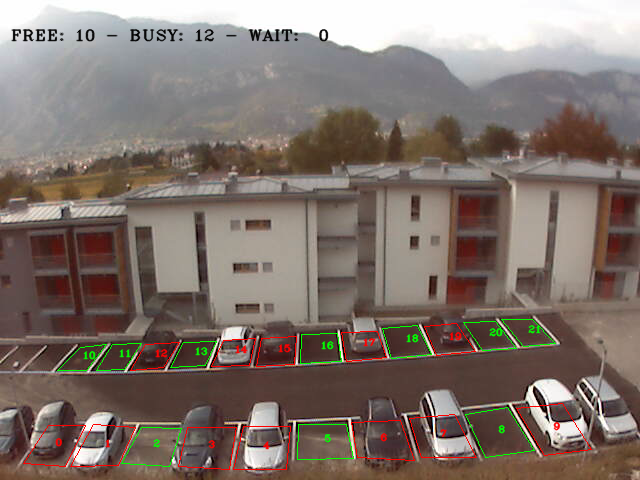
\includegraphics[keepaspectratio, scale=0.38]{img/ICbuffer.png}
	\caption{Image of the final result}
	\end{figure}


% Chapter 4: conclusions and further implementation

% \begin{thebibliography}{1}
% 
% \bibitem{springer_comp}
% D. E. Nilsson, M. F. Land, J. Howard,Optics of the butterfly eye, Journal of Comparative Physiology A, Volume 162, pp 341-366, 1988
% 
% \end{thebibliography}

\end{document}
